\section{Global Evaluator}

This global overview defines the baseline from which all subsequent power and precision trade-offs are derived.

\subsection*{Quantitative Results}
Table \ref{tab:global_benchmark} summarises the headline results for the G3 generation of the \texttt{DetectorNX} model architecture against its \gls{cnn} counterpart.

\begin{table}[H]
\centering
\resizebox{\textwidth}{!}{%
\begin{tabular}{|l|c|c|}
\hline
\textbf{Performance Metric} & \textbf{\texttt{DetectorNX-G3-SNN}} & \textbf{\texttt{DetectorNX-G3-CNN}} \\
\hline
Mean IoU & 0.4613 & 0.4861 \\
\gls{map_50} & 0.5977 & 0.6550 \\
Recall (Detections $>$ 0.5) & 100.0\% & 100.0\% \\
\hline
Avg.\ Detections per Frame (GT) & 2.02 & 2.02 \\
Avg.\ Detections per Frame (Pred) & 1.73 & 1.75 \\
\hline
Max Confidence & 0.9930 & 0.9918 \\
Min Confidence & 0.0011 & 0.0132 \\
\hline
\end{tabular}%
}
\caption{Global Performance Benchmark results for \texttt{DetectorNX-G3-SNN} and \texttt{DetectorNX-G3-CNN}, evaluated across the full 200-sample ETraM validation set \parencite{Verma_2024_CVPR}. Ground truth average detections per frame is 2.02 for both models by definition.}
\label{tab:global_benchmark}
\end{table}

\subsection*{Qualitative Results}

A qualitative audit was also conducted to visualise the models' spatial reasoning across the validation subset. Figure \ref{fig:qualitative_inference} illustrates the architectures' ability to resolve vehicle geometries in varied traffic conditions, providing the empirical context for the subsequent critical analysis of \gls{snn} precision. An expanded set of 20 paired samples is provided in Appendix~\ref{app:audit_samples}, with the full 200-sample audit available via the link given in Appendix~\ref{app:audit_samples}.

\begin{figure}[H]
    \centering
    \begin{subfigure}[b]{0.48\textwidth}
        \centering
        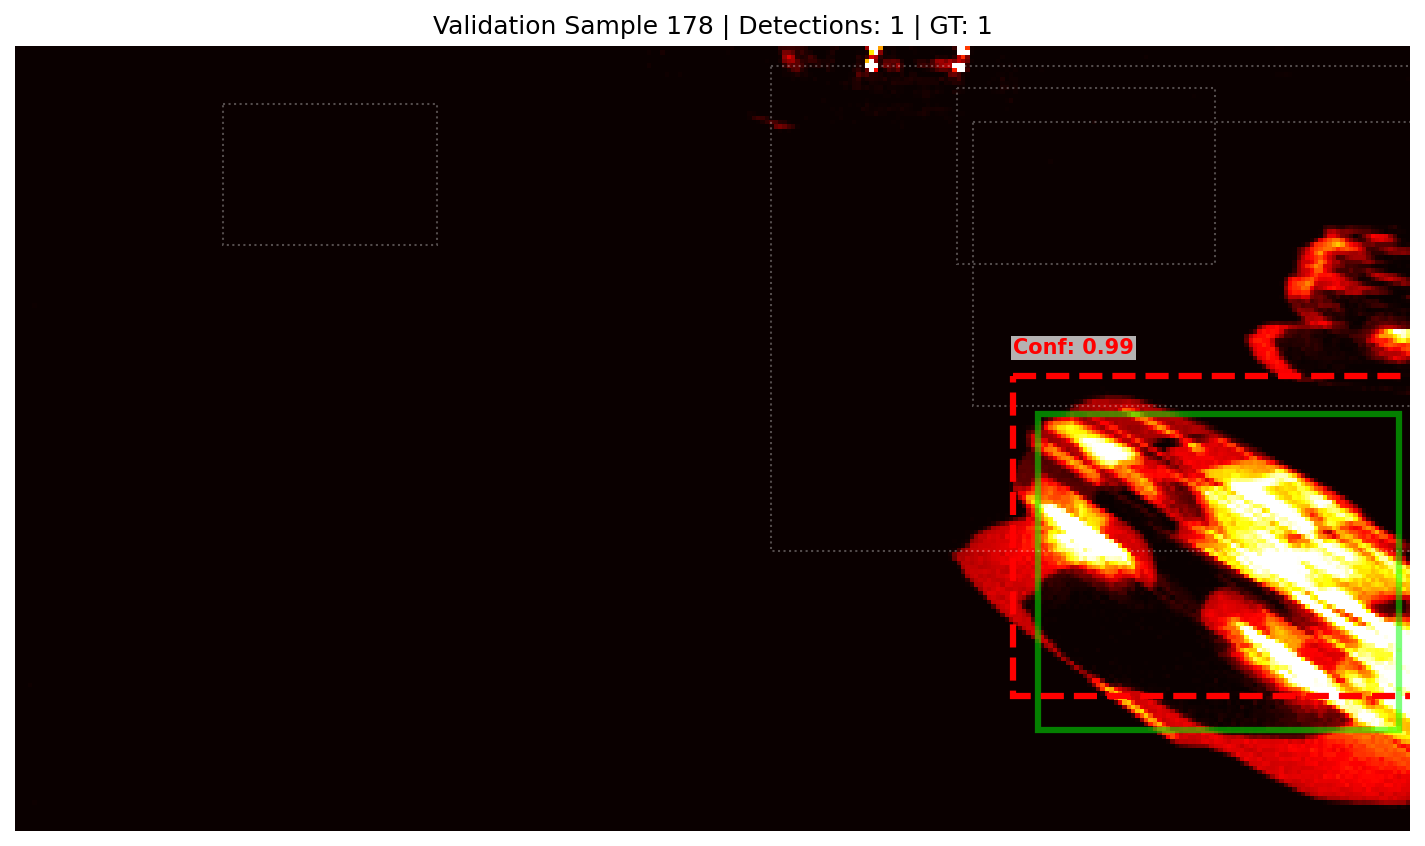
\includegraphics[width=\textwidth]{chapter_3/dnx_results/cnn_audit/audit_sample_178.png}
        \caption{CNN Baseline - Sample 178}
        \label{fig:cnn_sample178}
    \end{subfigure}
    \hfill
    \begin{subfigure}[b]{0.48\textwidth}
        \centering
        
\includegraphics[width=\textwidth]{chapter_3/dnx_results/snn_audit/audit_sample_178.png}
        \caption{SNN (G3) - Sample 178}
        \label{fig:snn_sample178}
    \end{subfigure}
    
    \vspace{1em}
    
    \begin{subfigure}[b]{0.48\textwidth}
        \centering
        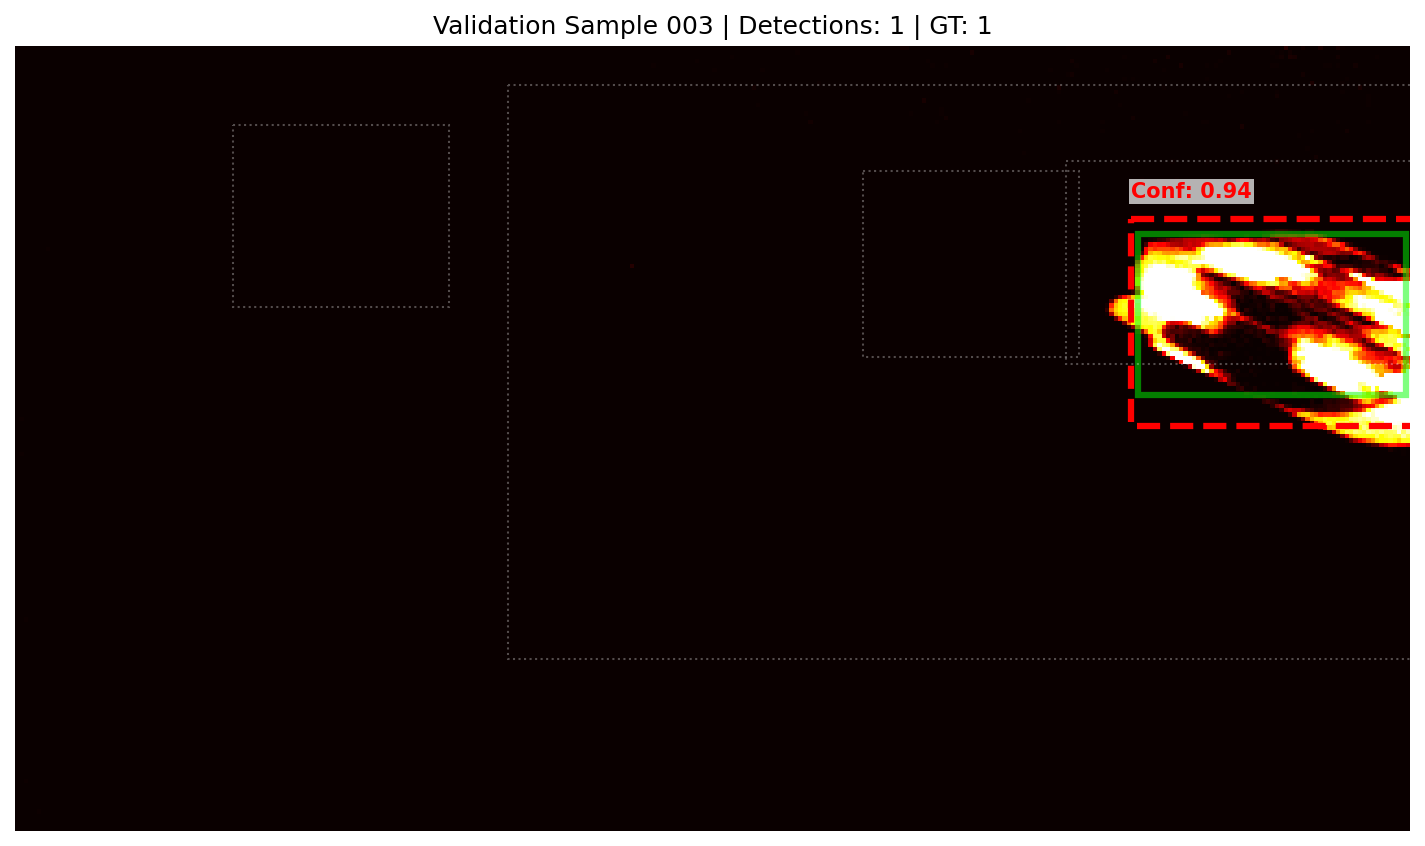
\includegraphics[width=\textwidth]{chapter_3/dnx_results/cnn_audit/audit_sample_003.png}
        \caption{CNN Baseline - Sample 003}
        \label{fig:cnn_sample003}
    \end{subfigure}
    \hfill
    \begin{subfigure}[b]{0.48\textwidth}
        \centering
        
\includegraphics[width=\textwidth]{chapter_3/dnx_results/snn_audit/audit_sample_003.png}
        \caption{SNN (G3) - Sample 003}
        \label{fig:snn_sample003}
    \end{subfigure}

    \vspace{1em}

    \centering
    \begin{subfigure}[b]{0.48\textwidth}
        \centering
        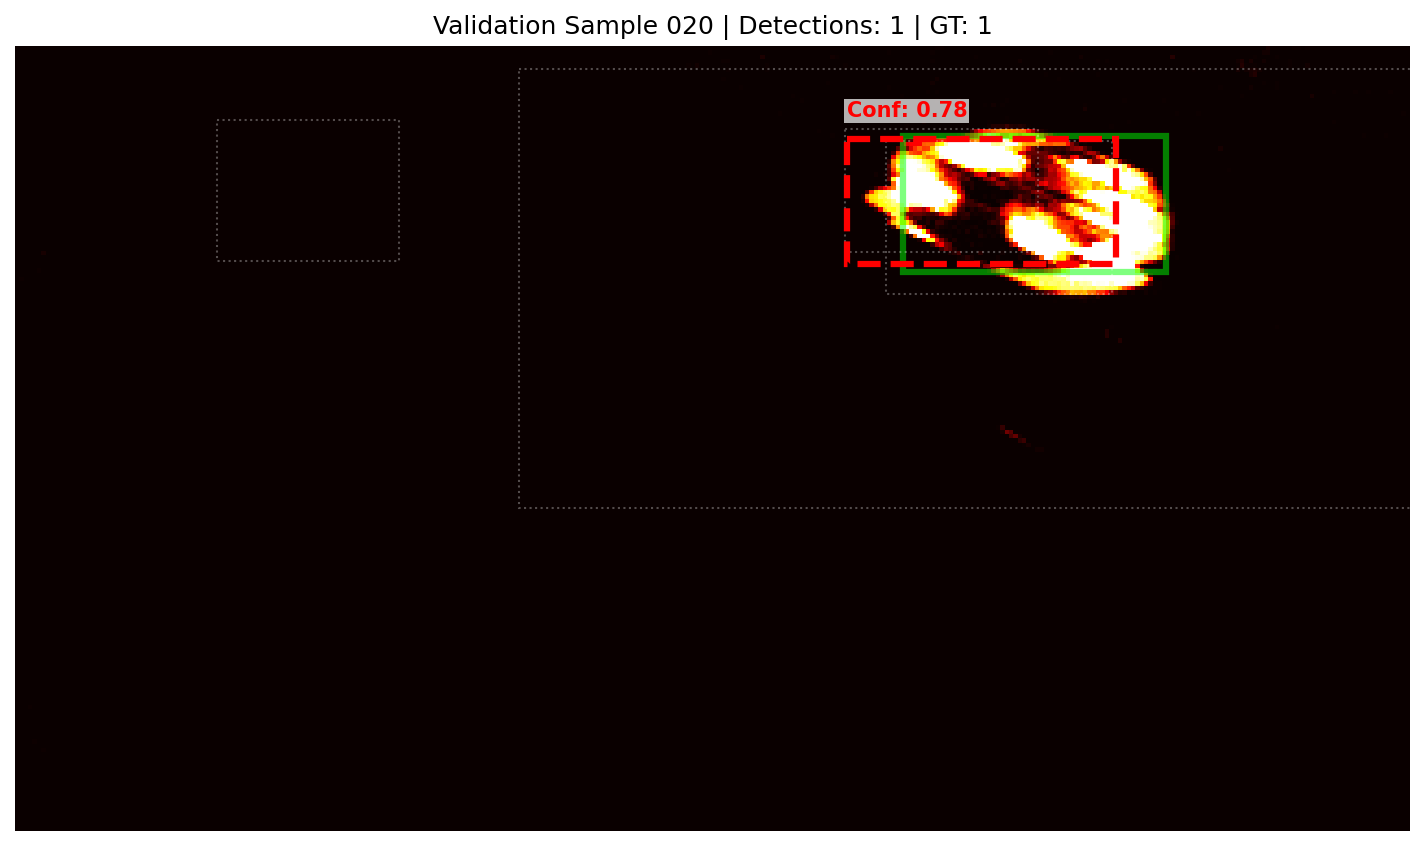
\includegraphics[width=\textwidth]{chapter_3/dnx_results/cnn_audit/audit_sample_020.png}
        \caption{CNN Baseline - Sample 020}
        \label{fig:cnn_sample020}
    \end{subfigure}
    \hfill
    \begin{subfigure}[b]{0.48\textwidth}
        \centering
        
\includegraphics[width=\textwidth]{chapter_3/dnx_results/snn_audit/audit_sample_020.png}
        \caption{SNN (G3) - Sample 020}
        \label{fig:snn_sample020}
    \end{subfigure}

    \caption[Qualitative Inference Audit]{Qualitative comparison of bounding box regression between the CNN baseline and SNN (G3) across representative validation samples.}
    \label{fig:qualitative_inference}
\end{figure}

\begin{figure}[H]
    \ContinuedFloat
    \centering
    
    \begin{subfigure}[b]{0.48\textwidth}
        \centering
        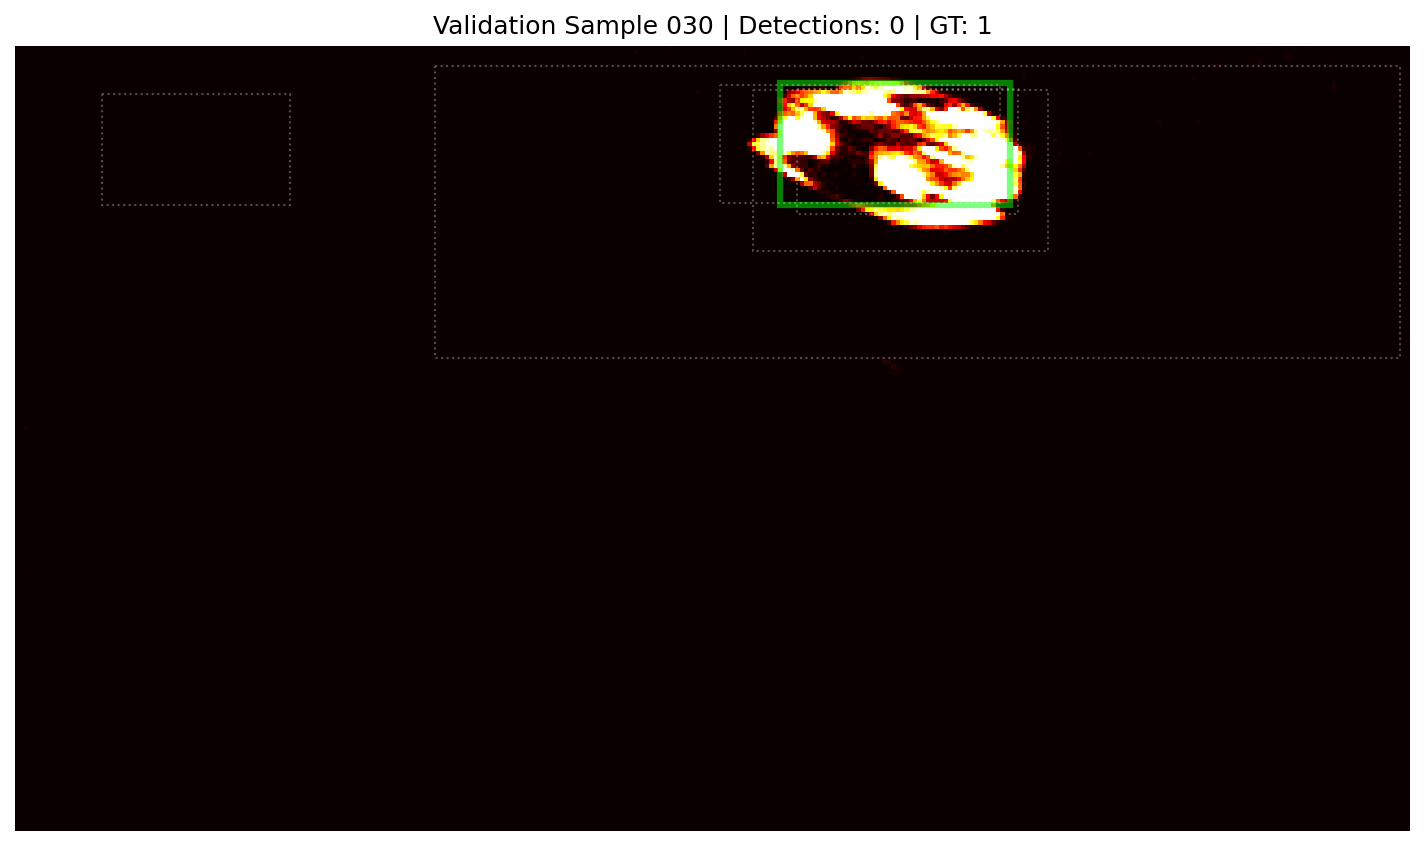
\includegraphics[width=\textwidth]{chapter_3/dnx_results/cnn_audit/audit_sample_030.png}
        \caption{CNN Baseline - Sample 030}
        \label{fig:cnn_sample030}
    \end{subfigure}
    \hfill
    \begin{subfigure}[b]{0.48\textwidth}
        \centering
        
\includegraphics[width=\textwidth]{chapter_3/dnx_results/snn_audit/audit_sample_030.png}
        \caption{SNN (G3) - Sample 030}
        \label{fig:snn_sample030}
    \end{subfigure}
    \caption[]{Qualitative comparison of bounding box regression between the CNN baseline and SNN (G3) across representative validation samples (continued).}
\end{figure}

\subsection*{Critical Analysis}

The results from Table \ref{tab:global_benchmark} demonstrate a remarkable degree of parity between the spiking and continuous paradigms. Achieving a mean \gls{iou} of $0.4613$, which corresponds to $94.9\%$ of the \gls{cnn} baseline, proves that the G3 backbone is robust enough to sustain high-resolution spatial reasoning despite the loss of precision inherent in $1$-bit quantisation. This geometric-precision parity is further corroborated by the detection-quality metric: the \gls{snn} achieves an \gls{map_50} of $0.5977$ against the \gls{cnn}'s $0.6550$, a $91.3\%$ parity under the stricter COCO-convention protocol that confirms the parity finding is not an artefact of the \gls{iou}-only evaluation. This parity indicates that the architectural refinements detailed in Section \ref{sec:architectural_evolution}---specifically the integration of \gls{se} blocks and \gls{sew} residual connections---have successfully compensated for the discrete nature of spiking activations.

This convergence in predictive capacity is further reflected in the detection metrics. Both models achieve a perfect recall of $100.0\%$ for objects with an IoU $> 0.5$, demonstrating that the transition to spiking dynamics has not induced any catastrophic forgetting of vehicle features. Furthermore, both models exhibit a similar detection profile compared to the ground truth ($1.73$ and $1.75$ predicted vs.\ $2.02$ ground truth average detections), which is typical for object detection on noisy, asynchronous event data. The negligible gap between the spiking and continuous variants confirms that the \gls{snn} has not compromised its feature extraction or proposal capacity.

Furthermore, the confidence distribution analysis provides the first indication of representational divergence. The \gls{snn} exhibits a lower minimum confidence ($0.0011$ vs.\ $0.0132$) compared to the baseline, while maintaining a competitive maximum confidence ($0.9930$ vs.\ $0.9918$). This suggests that the spiking model utilises a wider dynamic range of membrane potentials to differentiate between high-evidence targets and background noise. The ability of the \gls{snn} to suppress low-evidence detections more effectively than the continuous baseline points toward a more honest internal representation, a hypothesis further investigated in the calibration analysis (Section \ref{subsec:results_calibration}).

Qualitatively, Figure \ref{fig:qualitative_inference} confirms that the \gls{snn} maintains precise spatial alignment across diverse traffic densities. In Sample 178 and 030, the spiking model resolves vehicle clusters with the same degree of box stability as the \gls{cnn}, validating the effectiveness of the \texttt{DetectorNX} pipeline in preserving temporal context. In summary, the \texttt{DetectorNX-G3-SNN} has successfully bridged the precision gap, establishing a foundation for the subsequent evaluation of its power efficiency and temporal reliability.
